% ---------------------------- %
% Assignment Report Template
% 
% Heidi Christensen, 2020
% --------------------------   %


\documentclass[11pt,oneside]{article}
\usepackage[utf8]{inputenc}
\usepackage{graphicx}


\title{Experimental report for the 2021 COM1005 Assignment: The 8-puzzle Problem\footnote{Please, add here your \textsl{private} github url}}
\author{Your Name}
\date{\today}


\begin{document}

\maketitle

\section{Descriptions of my breadth-first and A* implementations}

\subsection{Breadth-first implementation}

Here I need to add an amazing description of my breadth-first implementation. This could include some screenshots of my code.

Figure~\ref{fig:panda} shows an example of how you include a picture in your report and how you give it a caption and a label that you can reference in the text.

\begin{figure}[ht]
\centering
  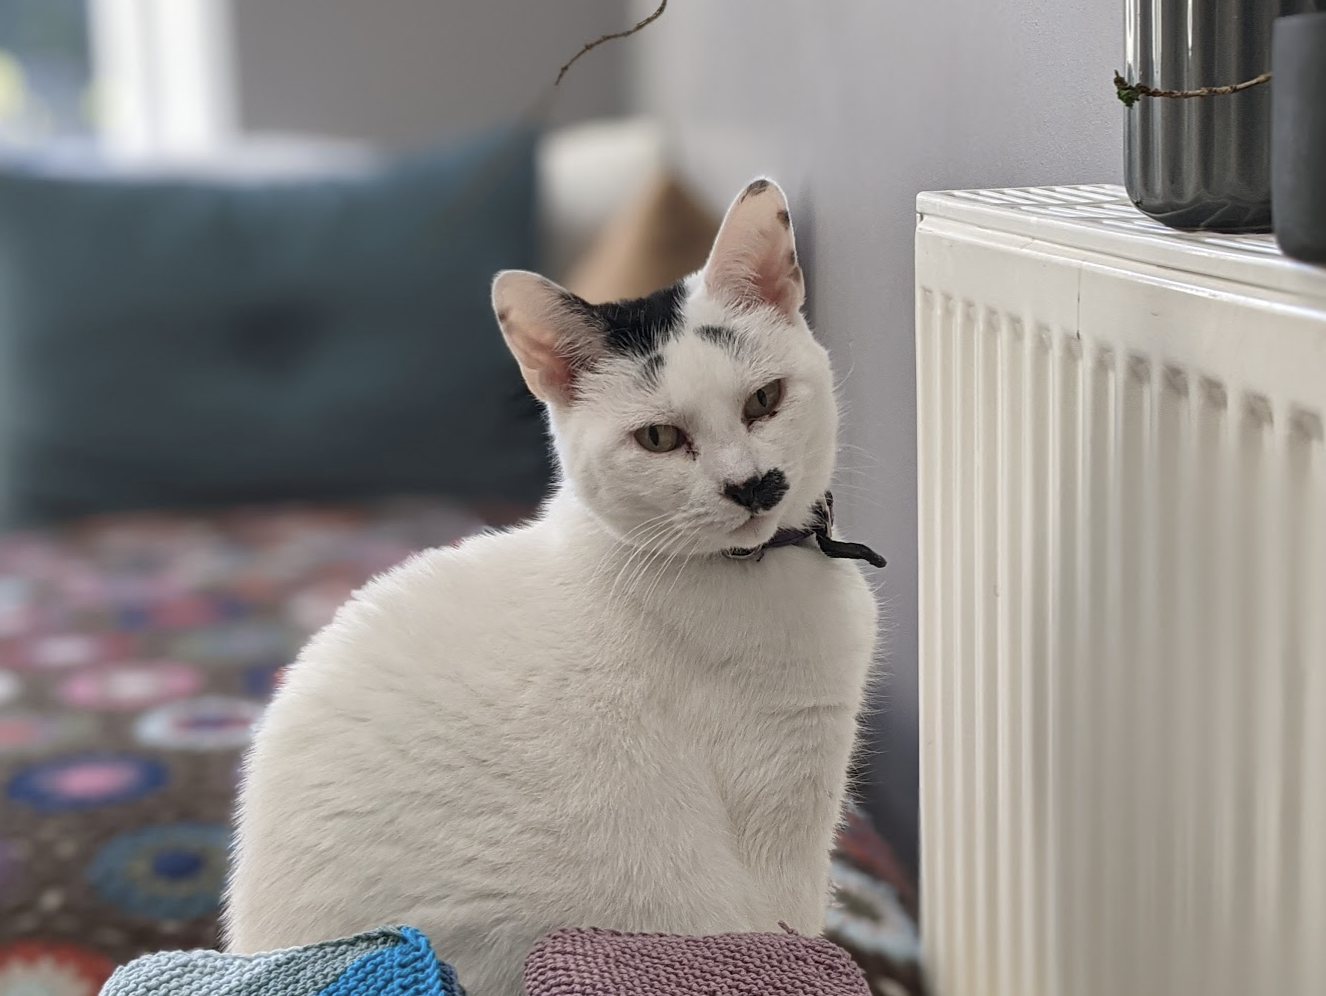
\includegraphics[scale=0.4]{Panda.png}
  \caption{This is Heidi's cat Panda.}
  \label{fig:panda}
 \end{figure} 

\subsection{A* implementation}

In this section I want to describe what I added to my classes to implement the A* search engine for the 8-puzzle problem. This should include a description of how I have implemented the two distance measures. Screenshots could also be great in this section.

This is an example of a list in \LaTeX. 

\begin{itemize}
    \item item 1.
    \item another great item.
\end{itemize}

\section{Results of assessing efficiency for the two search algorithms}

Here I will describe the results of the experiments I had to run to test my hypothsis.

Table~\ref{tab:my_label} shows something super important. This is an example of a table in \LaTeX\ and how you might reference it in the text.

\begin{table}[ht]
    \centering
    \begin{tabular}{|c|c|}
        System      & Measurement [\%] \\ \hline
        Basic       & 40\% \\
        Improved v1 & 42\% \\
        Improved v2 & 43\% \\
    \end{tabular}
    \caption{Example table}
    \label{tab:my_label}
\end{table}

 
\section{Conclusions}

Here I need to write what conclusions I can draw from my experimental work.


\end{document}
